\documentclass[11pt]{report}
\renewcommand{\baselinestretch}{1.5}


% Declaração dos pacotes
\usepackage[utf8]{inputenc}
\usepackage[T1]{fontenc}
\usepackage{graphicx}
\usepackage[portuguese]{babel}
\usepackage{graphicx}
\usepackage[affil-it]{authblk} % Usado para meter nome da escola
\usepackage{eurosym} % Usado para o €
\usepackage{url} % URL



% CAPA
\title{\textbf{\textit{Desenvolvimento de uma estação meteorológica em bare-metal e RTOS. }\\
		\large1º Trabalho prático de
		Sistemas Embebidos e de Tempo Real }}
			
				
\author{Rúben Guimarães nº11156\\ Kyrylo Yavorenko nº10355 }

\affil{Escola Superior de Tecnologia, IPCA \\
	Barcelos}	
	
		
\date{06 de Maio de 2018}


\begin{document}

\maketitle




% Indice
\tableofcontents


% Introdução
\chapter*{Introdução}
\addcontentsline{toc}{chapter}{Introdução}


O trabalho prático abordado neste relatório foi desenvolvido no âmbito da unidade curricular Sistemas Embebidos e de Tempo Real do curso de Engenharia de Sistemas Informáticos, lecionada pelo docente António Moreira. O docente desafiou os alunos a aplicarem os conceitos de programação de sistemas embebidos e de sistemas embebidos adquiridos durante o decorrer da unidade curricular. Desenvolvendo um projeto onde o desenvolvimento estivesse divido em duas partes (baremetal e e usando o sistema operativo FreeRTOS) e que adquirisse de diversas fontes de sinais analógicos e digitais para poder replicar o funcionamento de uma estação meteorológica.


\clearpage



% Resumo
\chapter*{Resumo}
\addcontentsline{toc}{chapter}{Resumo}

Neste trabalho desenvolvemos uma pequena estação meteorológica recorrendo a plataforma de prototipagem eletrónica open-source Arduino. Esta estação consiste num conjunto de sensores que obtém dados sobre o estado do tempo que depois são enviados para o Arduino para serem processados e por fim são mostrados ao utilizador quer através de um lcd de 16x2 quer através da consola do IDE do Arduino.


\clearpage


% Objectivos
\chapter*{Objectivos}
\addcontentsline{toc}{chapter}{Objectivos}

Os objetivos definidos para o projecto pelo docente foram:

\begin{itemize}
\item Desenvolvimento de um programa usando a tipologia baremetal.
\item Desenvolvimento de um programa usando o sistema operativo FreeRTOS usando 3 tasks.
\item Utilizar os seguintes sensores:
\begin{itemize}
\item Sensor de água.
\item 3 LDR's para calcular a posição do sol.
\item Sensor de humidade.
\item Dois sensores de temperatura (para o ar e o solo).
\item Barómetro.
\item Anemômetro 
\end{itemize}
\end{itemize}


\clearpage


% Arquitectura
\chapter*{Arquitectura}
\addcontentsline{toc}{chapter}{Arquitectura}

Podemos consultar na figura seguinte um diagrama com a arquitectura do projecto.


\begin{figure} [!h]
\centering
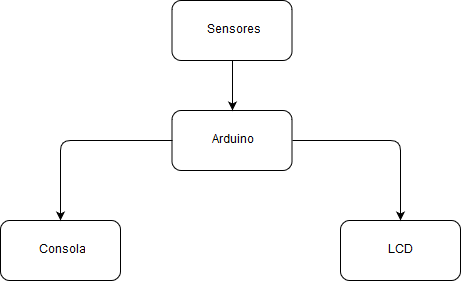
\includegraphics[width=\textwidth]{Prints/arquitectura.png}
\caption{Diagrama da arquitectura do projecto}
\label{Rotulo}
\end{figure}


\clearpage


% Recursos usados no projecto
\chapter*{Recursos usados no projecto}
\addcontentsline{toc}{chapter}{Recursos usados no projecto}

Para o desenvolvimento do projecto foram utilizados os seguintes recursos:

\textbf{Software:}
\begin{itemize}
\item \textit{Arduino IDE 18.5} para o desevolvimento do codigo usado.
\item \textit{GitHub Desktop} para atualizar o repositorio com o codigo do projecto.
\end{itemize}

\textbf{Hardware:}
\begin{itemize}
\item \textit{json2csharp} para a criação de classes dos ficheiros \textit{JSON}. \cite{json2csharp}
\item \textit{TinyTwitter} usada para facilitar a comunicação com o \textit{Twitter}.\cite{TinyTwitter}
\item \textit{Azure} usado para alojar o serviço e base de dados. \cite{TinyTwitter}
\end{itemize}



% API's externas usadas
\chapter*{API's externas usadas}
\addcontentsline{toc}{chapter}{API's externas usadas}

Foram usadas 4 API's externas:

\begin{itemize}
\item \textit{ipapi.co} - Usada para receber um ficheiro \textit{JSON} com as informações de um dado endereço IP.\cite{ipapi}
\item \textit{ipify  A  Simple IP Address API} - Usada para receber uma string com o endereço IP da nossa ligação.\cite{ipify}
\item \textit{Twitter Developer Platform} - Usada para publicar\textit{Tweets}  no \textit{Twitter}. \cite{twitter}
\item \textit{OpenWeatherMap} - Usada para receber um ficheiro \textit{JSON} com a informação meteologica de uma dada cidade. \cite{Weather}
\end{itemize}


% Desenvolvimento
\chapter*{Desenvolvimento}
\addcontentsline{toc}{chapter}{Desenvolvimento}

O serviço foi desenvolvido recorrendo a um serviço do tipo \textit{Windows Communication Foundation} (WCF). Este efetua a comunicação com as API's externas, trabalha os dados recebidos (se necessário) e disponibiliza serviços para um ou mais cliente usarem. Os serviços que disponibiliza são os seguintes:
\begin{itemize}
\item \textbf{GetIPInfo/\{enderecoIP\}} do tipo GET que envia a informação do endereço IP recebido no campo enderecoIP, num ficheiro \textit{JSON}
\item \textbf{MyIp} do tipo GET que envia a informação do endereço IP da ligação numa string.
\item \textbf{Tweet} do tipo POST que receber uma mensagem e publicar essa mensagem na conta \url{https://twitter.com/trabalhoisi}. Este recorre a uma biblioteca\cite{TinyTwitter} para facilitar a comunicação com o \textit{Twitter}.
\item \textbf{Weather/\{nomeCidade\}} do tipo GET que envia a informação metereologica da cidade recebida  no campo nomeCidade, num ficheiro \textit{JSON}
\end{itemize}

\clearpage

O serviço também contem objectos para guardar as respostas recebidas em \textit{JSON} criados no serviço \textit{json2csharp} tal como podemos verificar na imagem seguinte:



Este serviço atualmente esta publicado no \textit{Azure} e pode ser chamado usando o seguinte link \url{http://wcfrest20180109101801.azurewebsites.net/Service.svc/}.

\clearpage

O cliente foi  desenvolvido recorrendo ao \textit{Windows Presentation Foundation} (WPF) que recorre a linguagem de marcação \textit{Extensible Application Markup Language} (XAML) . Este é composto por 3 ambas (Endereços de IP/ Twitter / Meteorologia) onde existe uma interface onde podemos testar os serviços desevolvidos e ver os resultados. Podemos ver a aba do \textit{Twitter} na imagem seguinte.



% Conclução
\chapter*{Conclusão}
\addcontentsline{toc}{chapter}{Conclusão}

Este trabalho permitiu-se aplicar os conhecimentos adquiridos durante o desenrolar da unidade curricular de Integração de Sistemas de Informação e explorar e desenvolver processos de interoperabilidade entre sistemas, assentes em serviços web. Uma das partes que correu mal no trabalho foi o uso da base de dados alojada no \textit{Azure} que por algum motivo não mantinha a ligação aberta quando a tentava usar no serviço. De qualquer forma acho que este trabalho foi um sucesso tendo conseguido alcançar os meus objetivos e ficando a conheçer mais sobre serviços RESTful.

% Bilbiografia
\begin{thebibliography}{2}

	\bibitem{json2csharp}
	\emph{json2csharp }.  01 Janeiro, 2018. 
	\url{http://json2csharp.com/}


	\bibitem{TinyTwitter}
	jmhdez. \emph{TinyTwitter}.  01 Janeiro, 2018. 
	\url{https://github.com/jmhdez/TinyTwitter}


	\bibitem{Azure}
	\emph{Azure}.  01 Janeiro, 2018. 
	\url{https://portal.azure.com/}


	\bibitem{ipapi}
	\emph{ipapi.co}.  01 Janeiro, 2018. 
	\url{https://ipapi.co/}


	\bibitem{ipify}
	\emph{ipify} A Simple IP Address API.  01 Janeiro, 2018. 
	\url{https://www.ipify.org/}


	\bibitem{twitter}
	\emph{Twitter} Developer Platform.  03 Janeiro, 2018. 
	\url{https://developer.twitter.com/}


	\bibitem{Weather}
	\emph{OpenWeatherMap} Current weather and forecasts in your city.  05 Janeiro, 2018. 
	\url{http://openweathermap.org/current}
	

\end{thebibliography}
\addcontentsline{toc}{chapter}{Bibliografia}

\end{document}